\section{Marco teórico}

Entre las fuerzas ejercidas a la gota de aceite se encuentran la fuerza gravitacional $\Vec{\omega}$, la fuerza asociada al empuje o flotabilidad descrito por el principio de Arquimedes $\Vec{F}_b$ y la fuerza de fricción generada por el aire $\Vec{F}_D$ descrito por la ley de Stokes.\\

\begin{figure}
    \centering
    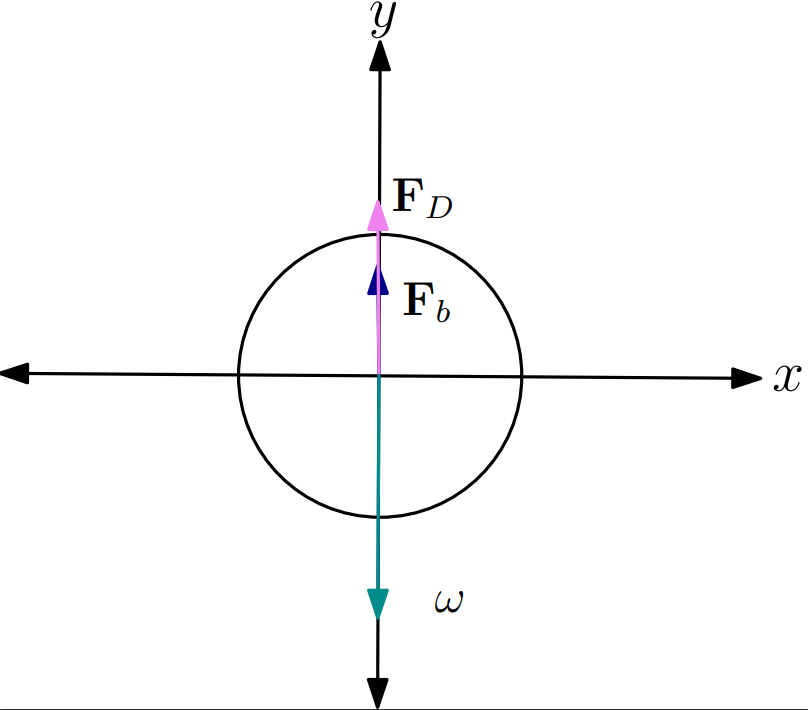
\includegraphics[width=0.5\linewidth]{Images/dcl_bajada.png}
    \caption{Diagrama de cuerpo libre de la gota de aceite en el primer intervalo de tiempo}
    \label{fig:enter-label}
\end{figure}

Inicialmente la gota es acelerada en dirección a la tierra pero prontamente llega a una velocidad terminal, esto indica un equilibrio de fuerzas.

\begin{equation}
    \begin{split}
        \sum \Vec{F}=0\\
        \lvert \Vec{F}_D\rvert + \lvert\Vec{F}_b\rvert + \lvert \Vec{\omega}\rvert =0
    \end{split}
\end{equation}

La fuerza de la gravedad, flotación y fricción se describen en la ecuación \cref{eq:bouyant-force} en donde $V_{ac}$ representa el volumen de la gota de aceite y $\mu$ es el coeficiente de viscosidad del aire:

\begin{equation}\label{eq:forces}
    \begin{split}
        \Vec{\omega}=m\Vec{g}\\
        \Vec{F}_b=-\rho_a \Vec{g}V_{ac}\\
        \Vec{F}_D=-6\pi r\mu \Vec{v}_c
    \end{split}
\end{equation}

Tomando en cuenta únicamente las magnitudes y remplazando se encuentra

\begin{equation}
    6\pi r\mu v_c=mg-\rho_a \Vec{g}V_{ac}
\end{equation}

Debido a que no se mide la masa de la gota, se dejará el volumen $V_{ac}$ y la masa $m$ en términos de su radio $r$ utilizando las ecuaciones \cref{eq:bouyant-volume} 

\begin{equation}\label{eq:volume}
    \begin{split}
        V_{ac}=\frac{4}{3}\pi r^3\\
        m=\frac{4}{3}\pi r^3\rho_{ac}
    \end{split}
\end{equation}

Remplazando y operando se obtiene

\begin{equation}
    \begin{split}
        6\pi r\mu v_c=\frac{4}{3}\pi r^3(\rho_{ac}-\rho_a)g
    \end{split}
\end{equation}

de la cual se obtiene el valor para $r$

\begin{equation}
    \begin{split}
        r=\sqrt{\frac{9\mu v_c}{2g(\rho_{ac}-\rho_a)}}
    \end{split}
\end{equation}

Para el segundo intervalo de tiempo, se aplica una diferencia de potencial y la gota empieza a ascender hacia la placa superior, nuevamente al llegar a la velocidad terminal, esta vez llamada $v_a$ ocurre un equilibrio de fuerzas en donde $\Vec{F}_e$ es la fuerza eléctrica.

\begin{figure}
    \centering
    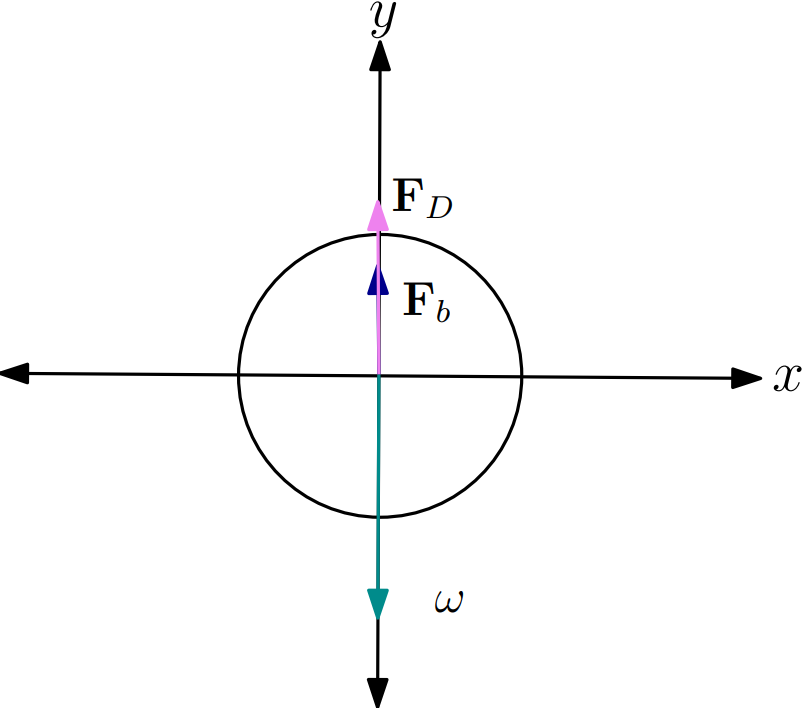
\includegraphics[width=0.5\linewidth]{Images/dcl_subida.png}
    \caption{Diagrama de cuerpo libre de la gota de aceite en el segundo intervalo de tiempo}
    \label{fig:enter-label}
\end{figure}

Las ecuaciones para el diagrama de cuerpo libre son \cref{eq:forces2} 

\begin{equation} \label{eq:forces2}
    \begin{split}
        \lvert\Vec{F}_b\rvert + \lvert \Vec{F}_e\rvert + \lvert \Vec{\omega}\rvert+\lvert \Vec{F}_D\rvert =0
    \end{split}
\end{equation}

Nuevamente se utilizan solo sus magnitudes, remplazando $F_e=qE$ donde $E$ es el campo eléctrico y operando se obtiene

\begin{equation}
    \begin{split}
        qE=6\pi r\mu v_a + \frac{4}{3}\pi r^3(\rho_{ac}-\rho_a)
    \end{split}
\end{equation}

utilizando la ecuación que relaciona la fuerza de fricción con la fuerza de la gravedad y de flotabilidad, además de remplazar el campo electrico por su expresión en un capacitor $E=\frac{V}{d}$ se llega a que la expresión para la carga en la gota es:

\begin{equation}
    \begin{split}
        q=\frac{6\pi \mu d}{V}\sqrt{\frac{9\mu v_c}{2g(\rho_{ac}-\rho_a)}}(v_a-v_c)
    \end{split}
\end{equation}i

Por último, sabemos que la carga está cuantizada y debe ser múltiplo de un valor $e^-$ en dónde $n$ es el número de electrones en la gota y se cumple la relación

\begin{equation}
    q=ne^-
\end{equation}
